\documentclass[12pt, letterpaper]{article}
%\documentclass[a4paper,12pt]{article}

%% Language and font encodings
\usepackage[english]{babel}
\usepackage[utf8x]{inputenc}
\usepackage[T1]{fontenc}
\usepackage{ amssymb }
\usepackage{ mathrsfs }
\usepackage{indentfirst}
\setlength{\parindent}{4ex}

%% Sets page size and margins
\usepackage[a4paper,top=3cm,bottom=2cm,left=3cm,right=3cm,marginparwidth=1.75cm]{geometry}

%% Useful packages
\usepackage{amsmath}
\usepackage{graphicx}
\usepackage[colorinlistoftodos]{todonotes}
\usepackage[colorlinks=true, allcolors=blue]{hyperref}
\usepackage{amsthm}
\usepackage{booktabs}
\numberwithin{equation}{section}
\theoremstyle{definition}
\newtheorem{remark}{Axiom}


\title{Write-Up of Stata Practice}
\author{Daniel Banko \thanks{The author would like to thank the CFPB and his parents for their love and support.}}
\date{November 2017}
\begin{document}
\begin{titlepage}
\maketitle
\end{titlepage}
\section{Introduction}
\subsection{Background}
\subsubsection{Subsubsection}
\indent
\\
%\todo[inline, color=green!40]{This is an inline comment.}

\begin{figure}
\centering
%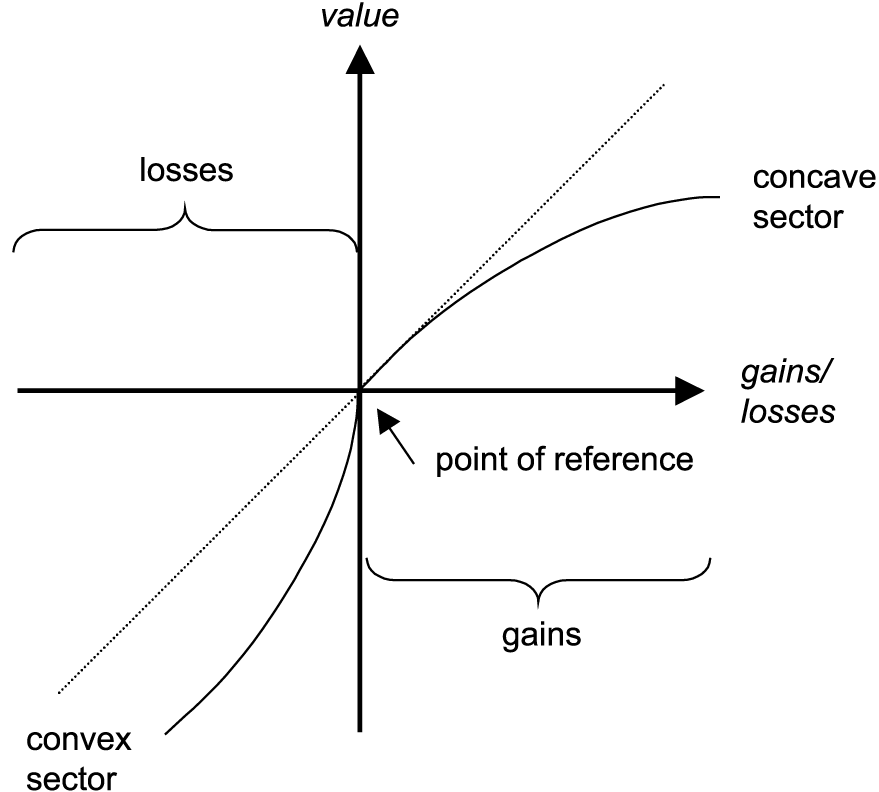
\includegraphics[width=0.7\textwidth]{prospect_theory.png}
%\caption{\label{fig:valuefunction} Prospect theory value function.}
\end{figure}

\begin{eqnarray*}
\end{eqnarray*}


\begin{table}
\input{../tables/"table1_regress_noshow_sms.tex"}
\caption{\label{tab:widgets}An example table.}
\end{table}

\begin{enumerate}
\item Like this,
\item and like this.
\end{enumerate}
\dots or bullet points \dots
\begin{itemize}
\item Like this,
\item and like this.
\end{itemize}

\section{References}
\subsection{How to add Citations and a References List}

You can upload a \verb|.bib| file containing your BibTeX entries, created with JabRef; or import your \href{https://www.overleaf.com/blog/184}{Mendeley}, CiteULike or Zotero library as a \verb|.bib| file. You can then cite entries from it, like this: \cite{greenwade93}. Just remember to specify a bibliography style, as well as the filename of the \verb|.bib|.

You can find a \href{https://www.overleaf.com/help/97-how-to-include-a-bibliography-using-bibtex}{video tutorial here} to learn more about BibTeX.

We hope you find Overleaf useful, and please let us know if you have any feedback using the help menu above --- or use the contact form at \url{https://www.overleaf.com/contact}!

\bibliographystyle{alpha}
\bibliography{sample}

\noindent
\hangindent=0.7cm
Tversky, Amos and Daniel Kahneman. "Advances in Prospect Theory: Cumulative Representation of Uncertainty." Journal of Risk and Uncertainty, 5.4 (1992): 297-323.\\

\noindent
\hangindent=0.7cm
Kahneman, Daniel and Amos Tversky. "Prospect Theory: An Analysis of Decision under Risk." Econometrica, 47.2 (1979): 263-292.?\\

\end{document}